%!TEX root = ../template.tex
%%%%%%%%%%%%%%%%%%%%%%%%%%%%%%%%%%%%%%%%%%%%%%%%%%%%%%%%%%%%%%%%%%%%
%% appendix1.tex
%% NOVA thesis document file
%%
%% Chapter with example of appendix with a short dummy text
%%%%%%%%%%%%%%%%%%%%%%%%%%%%%%%%%%%%%%%%%%%%%%%%%%%%%%%%%%%%%%%%%%%%

\typeout{NT FILE appendix1.tex}%

\begin{comment}

\chapter{Tipos de Dashboards}
\label{app:tipos_dashboards_app}

\begin{figure}[htbp]
  \begin{subfigure}{0.5\textwidth}
    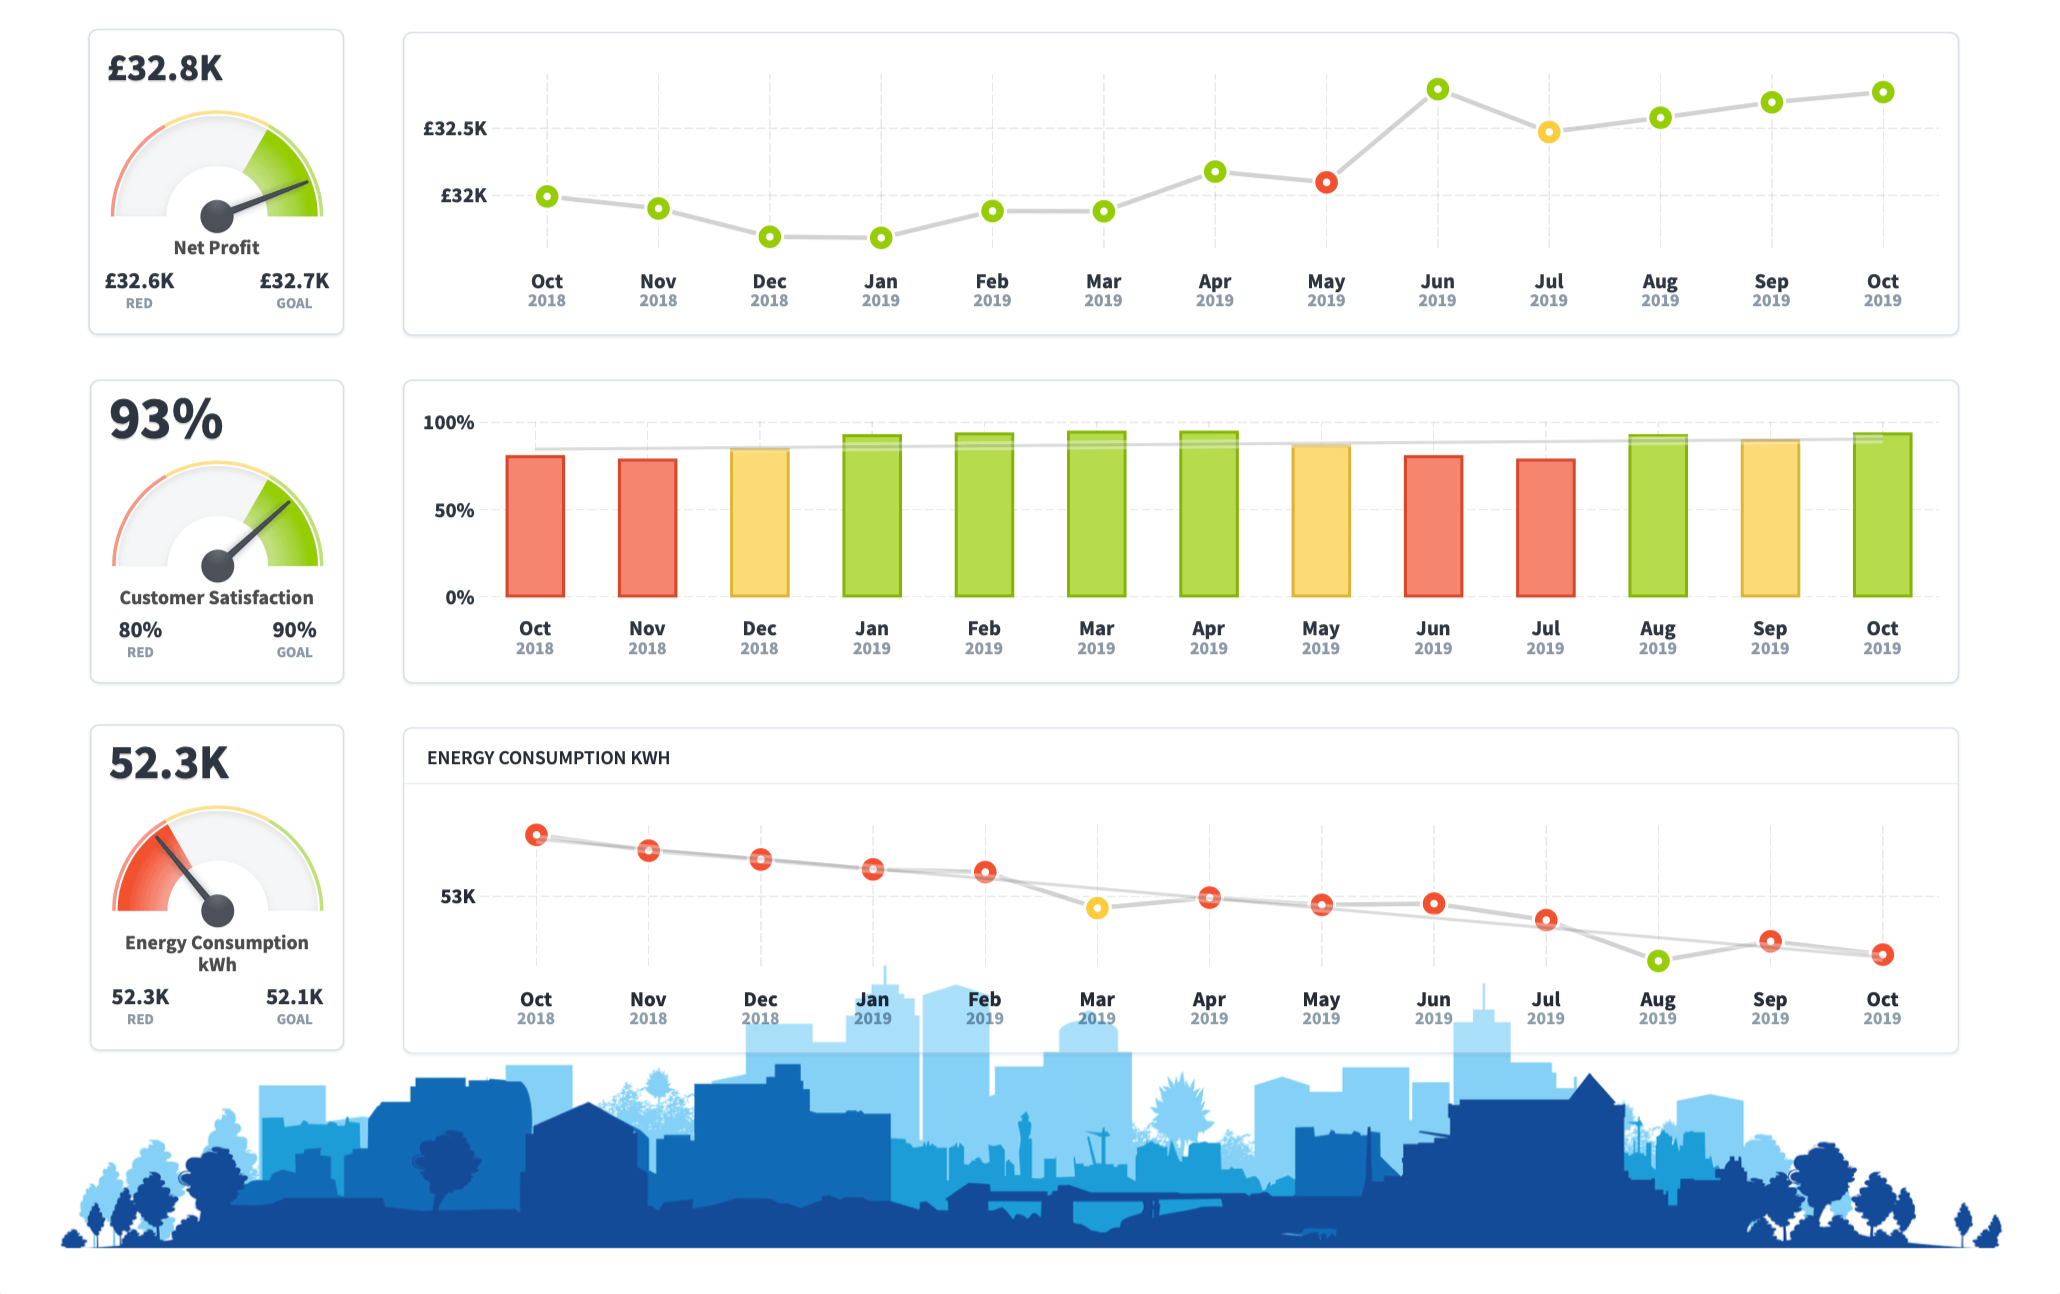
\includegraphics[width=0.9\linewidth, height=5cm]{strategic-dashboard.png} 
    \caption{Exemplo de um \textit{dashboard} estratégico \cite{IntrafocusKPIDashboard}.}
    \label{fig:strat-dash}
  \end{subfigure}
  \begin{subfigure}{0.5\textwidth}
    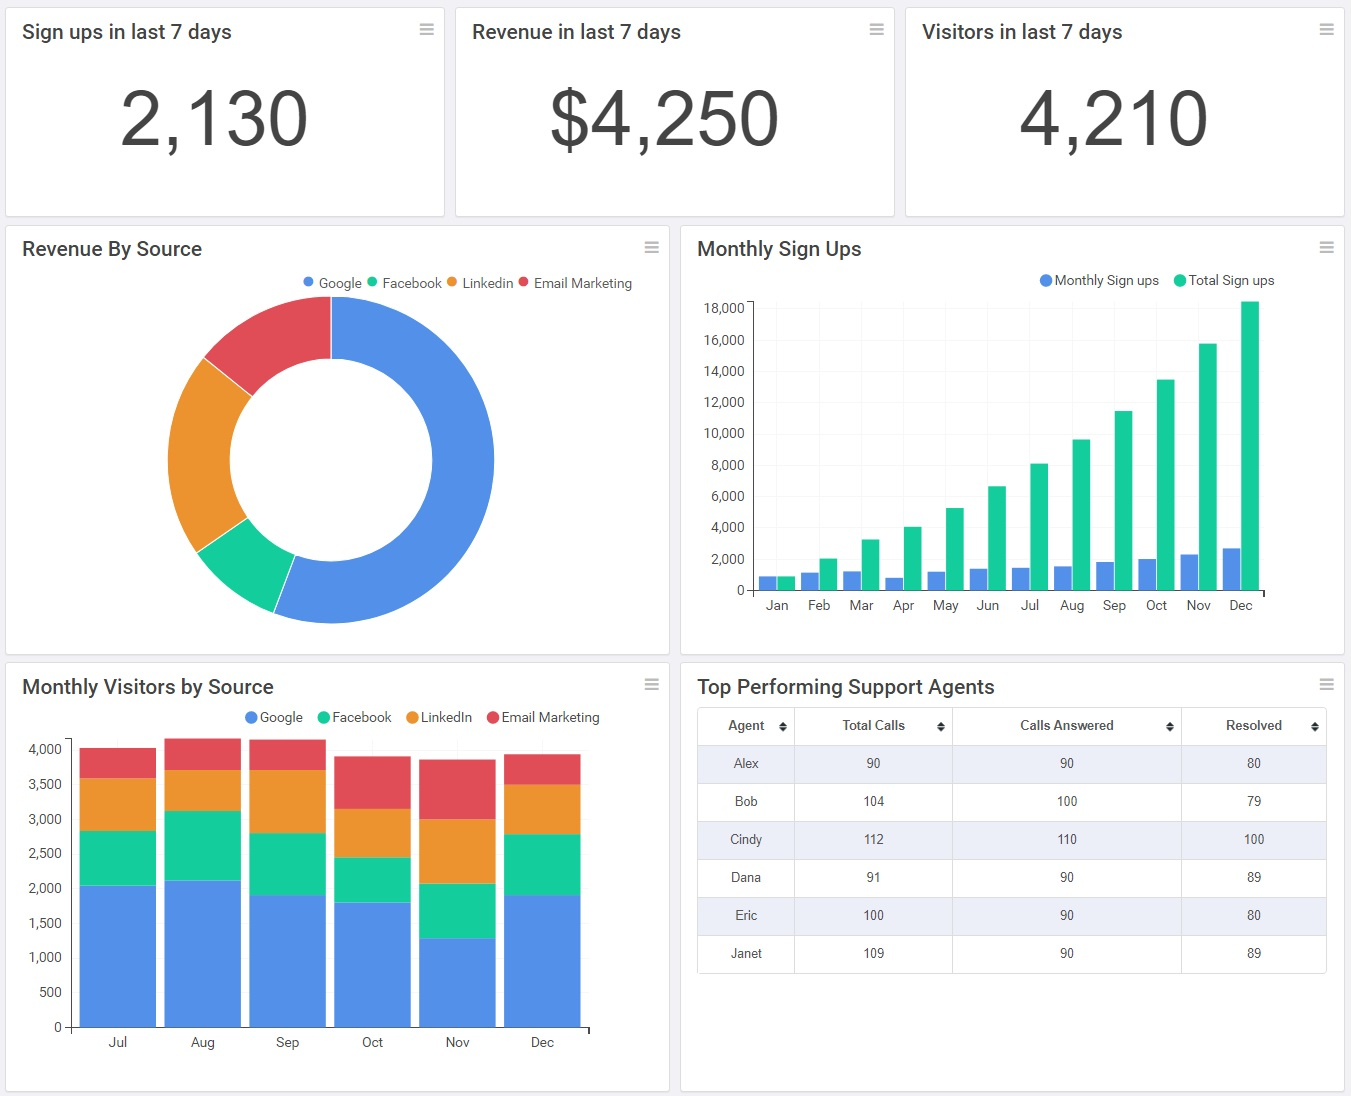
\includegraphics[width=0.9\linewidth, height=5cm]{operational-dashboard.jpg}
    \caption{Exemplo de um \textit{dashboard} operacional \cite{RegendusPowerBIAlternatives}.}
    \label{fig:op-dash}
  \end{subfigure}
  \begin{subfigure}{0.5\textwidth}
    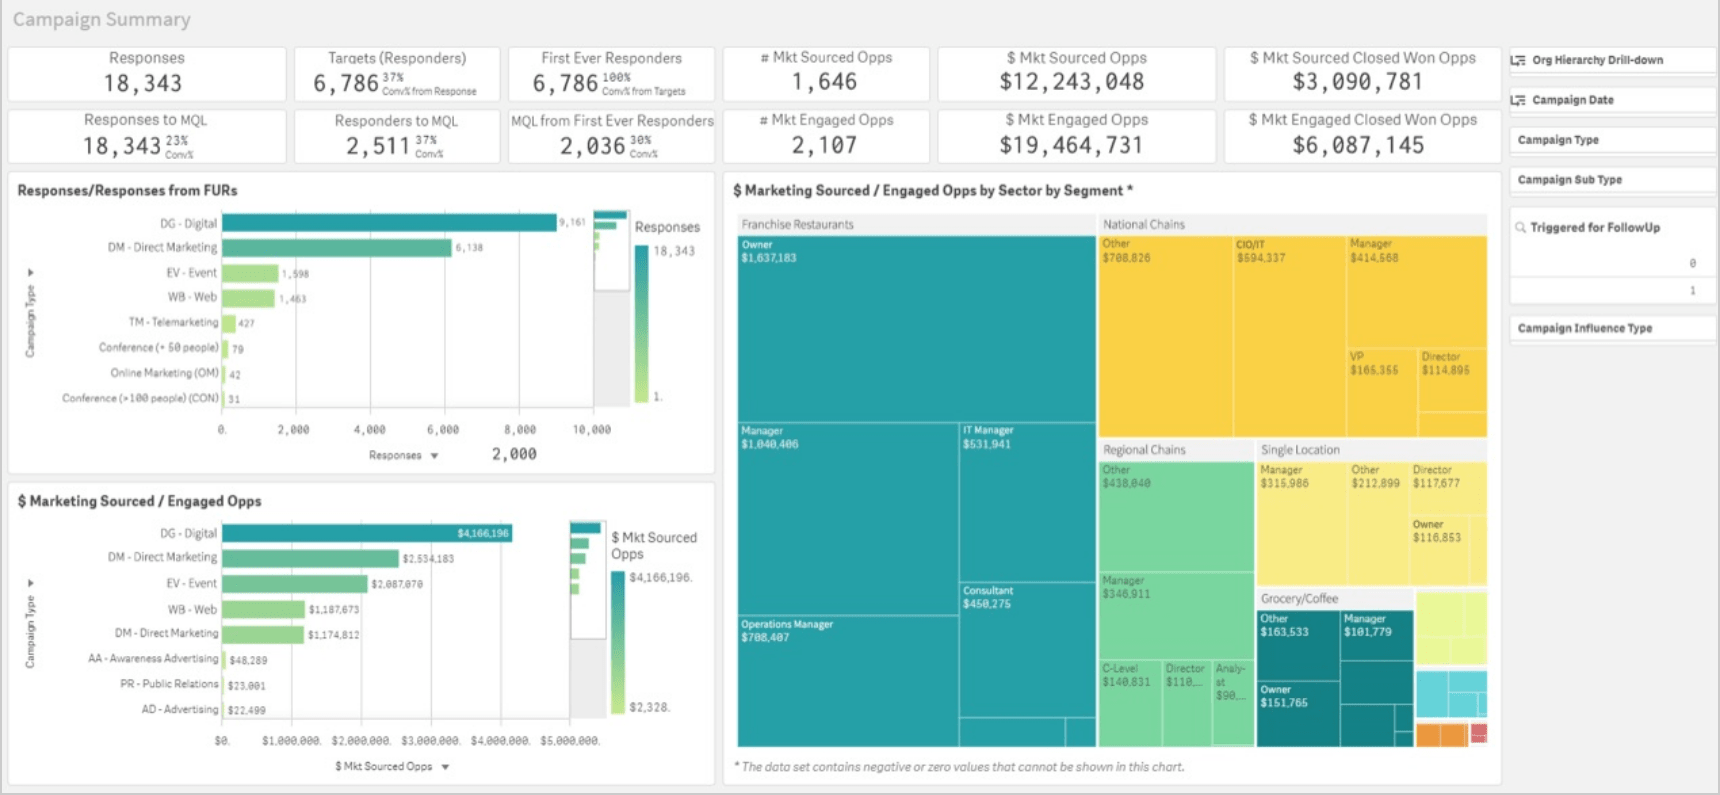
\includegraphics[width=0.9\linewidth, height=5cm]{analytical-dashboard3-remake.png}
    \caption{Exemplo de um \textit{dashboard} analítico \cite{QlikAnalyticsDashboard}.}
    \label{fig:anal-dash}
  \end{subfigure}
  
  \caption{Diferentes tipos de \textit{Dashboards}}
  \label{fig:image2}
\end{figure}

\end{comment}

\chapter{Meta-modelo}
\label{app:meta_modelo_app}

\begin{figure}[htbp]
  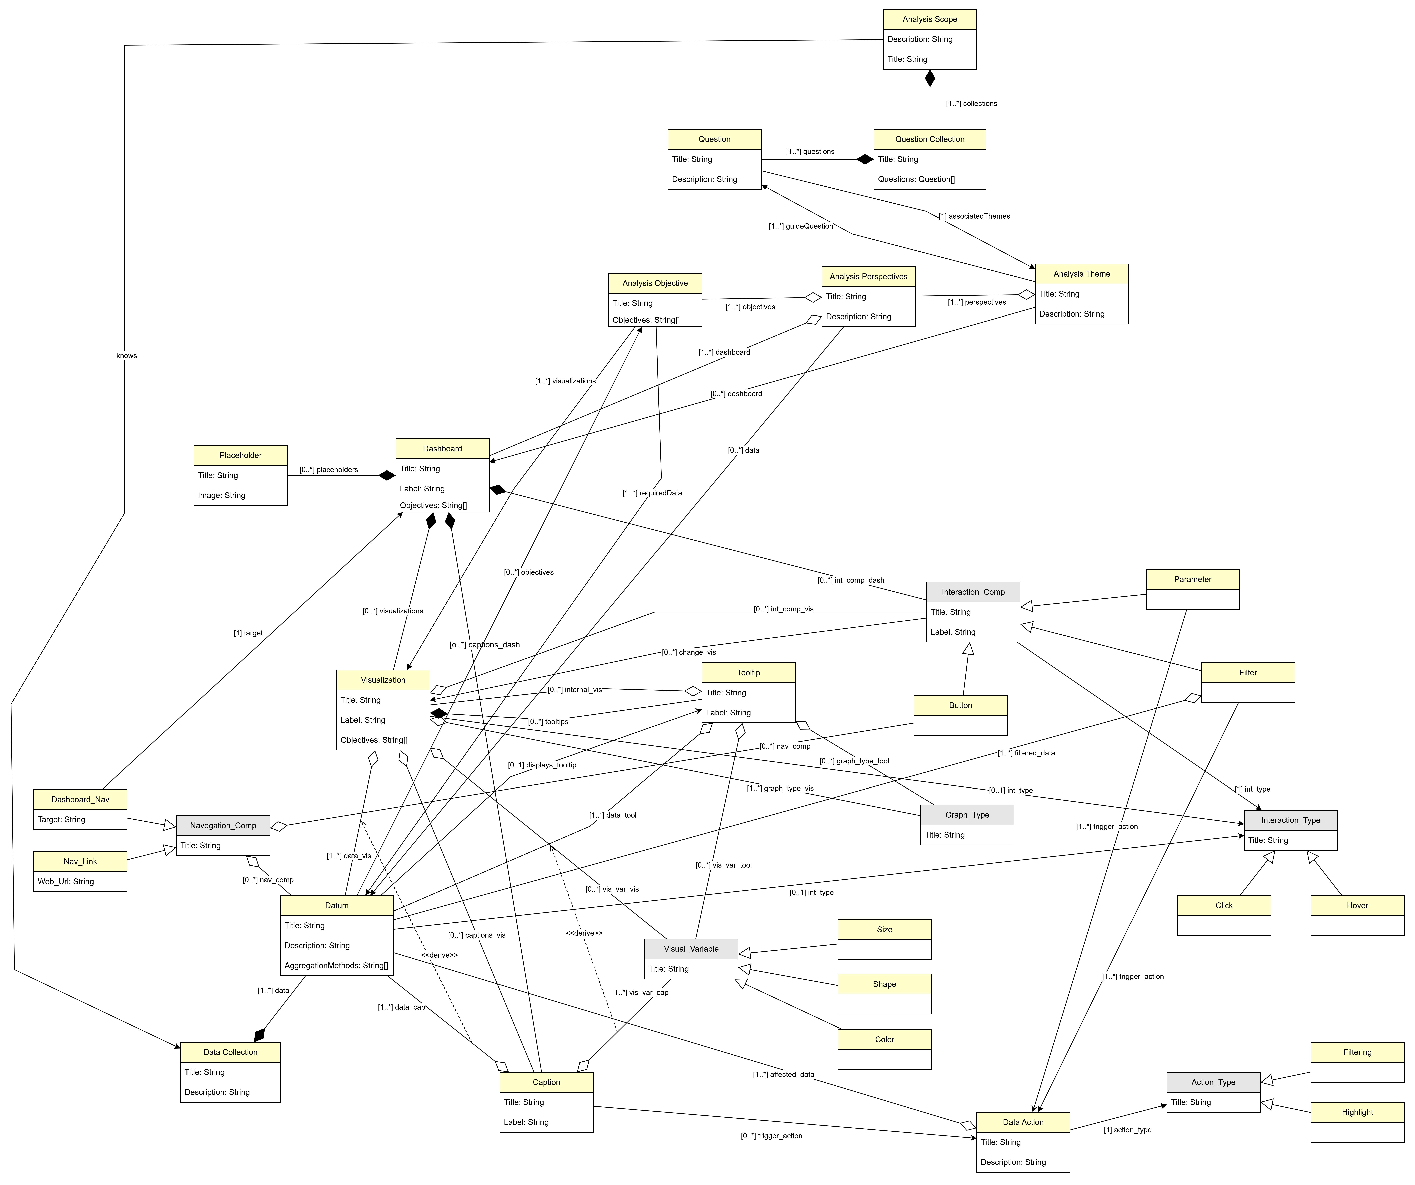
\includegraphics[width=\textwidth]{meta_modelo/completeDiagram_cropped}
  \centering
  \caption{Meta-modelo completo.}
  \label{fig:meta_modelo_img}
\end{figure}

\chapter{Protótipo inicial}
\label{app:prototipo_inicial}

\begin{figure}[htbp]
  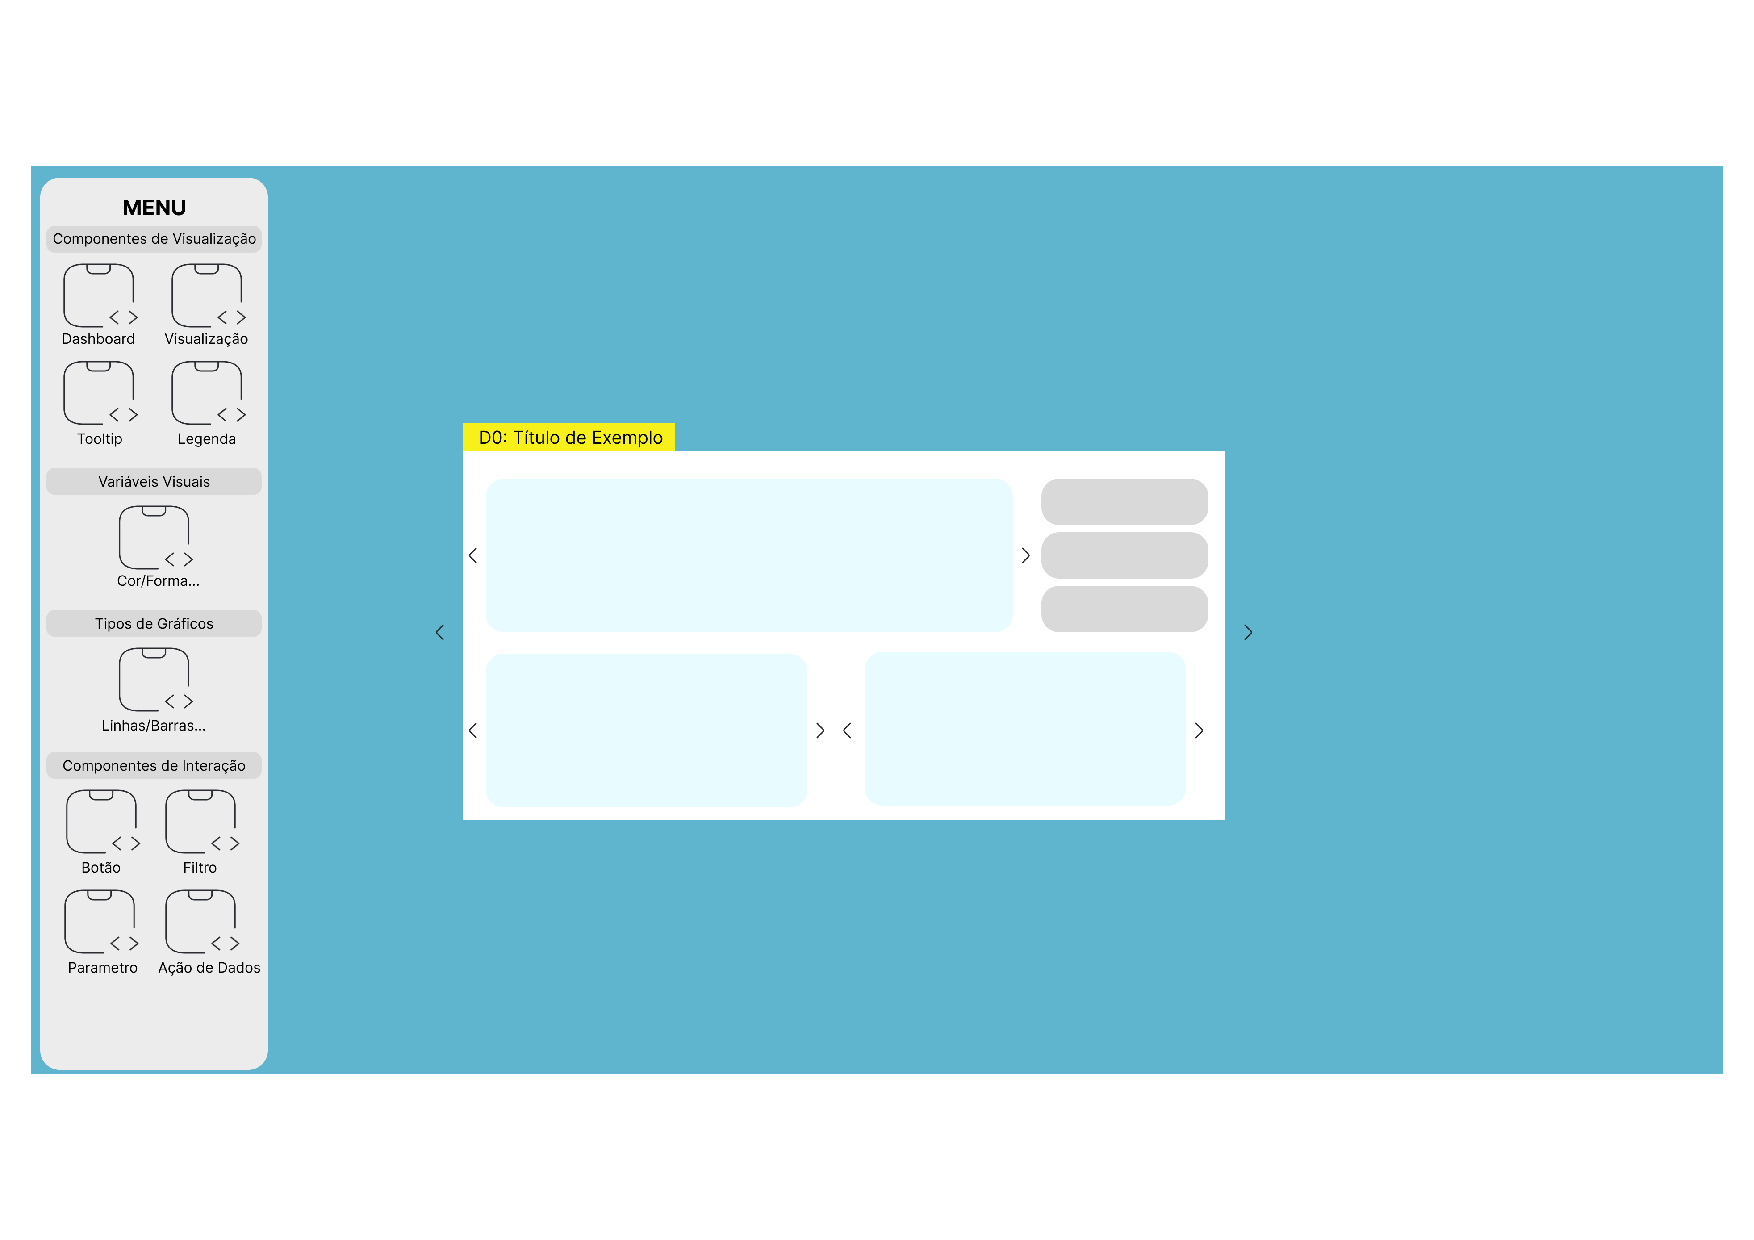
\includegraphics[height=4in]{prototipo/prototipo_desktop}
  \centering
  \caption{Protótipo da interface da ferramenta.}
  \label{fig:prototipo_desktop}
\end{figure}

\begin{figure}[htbp]
  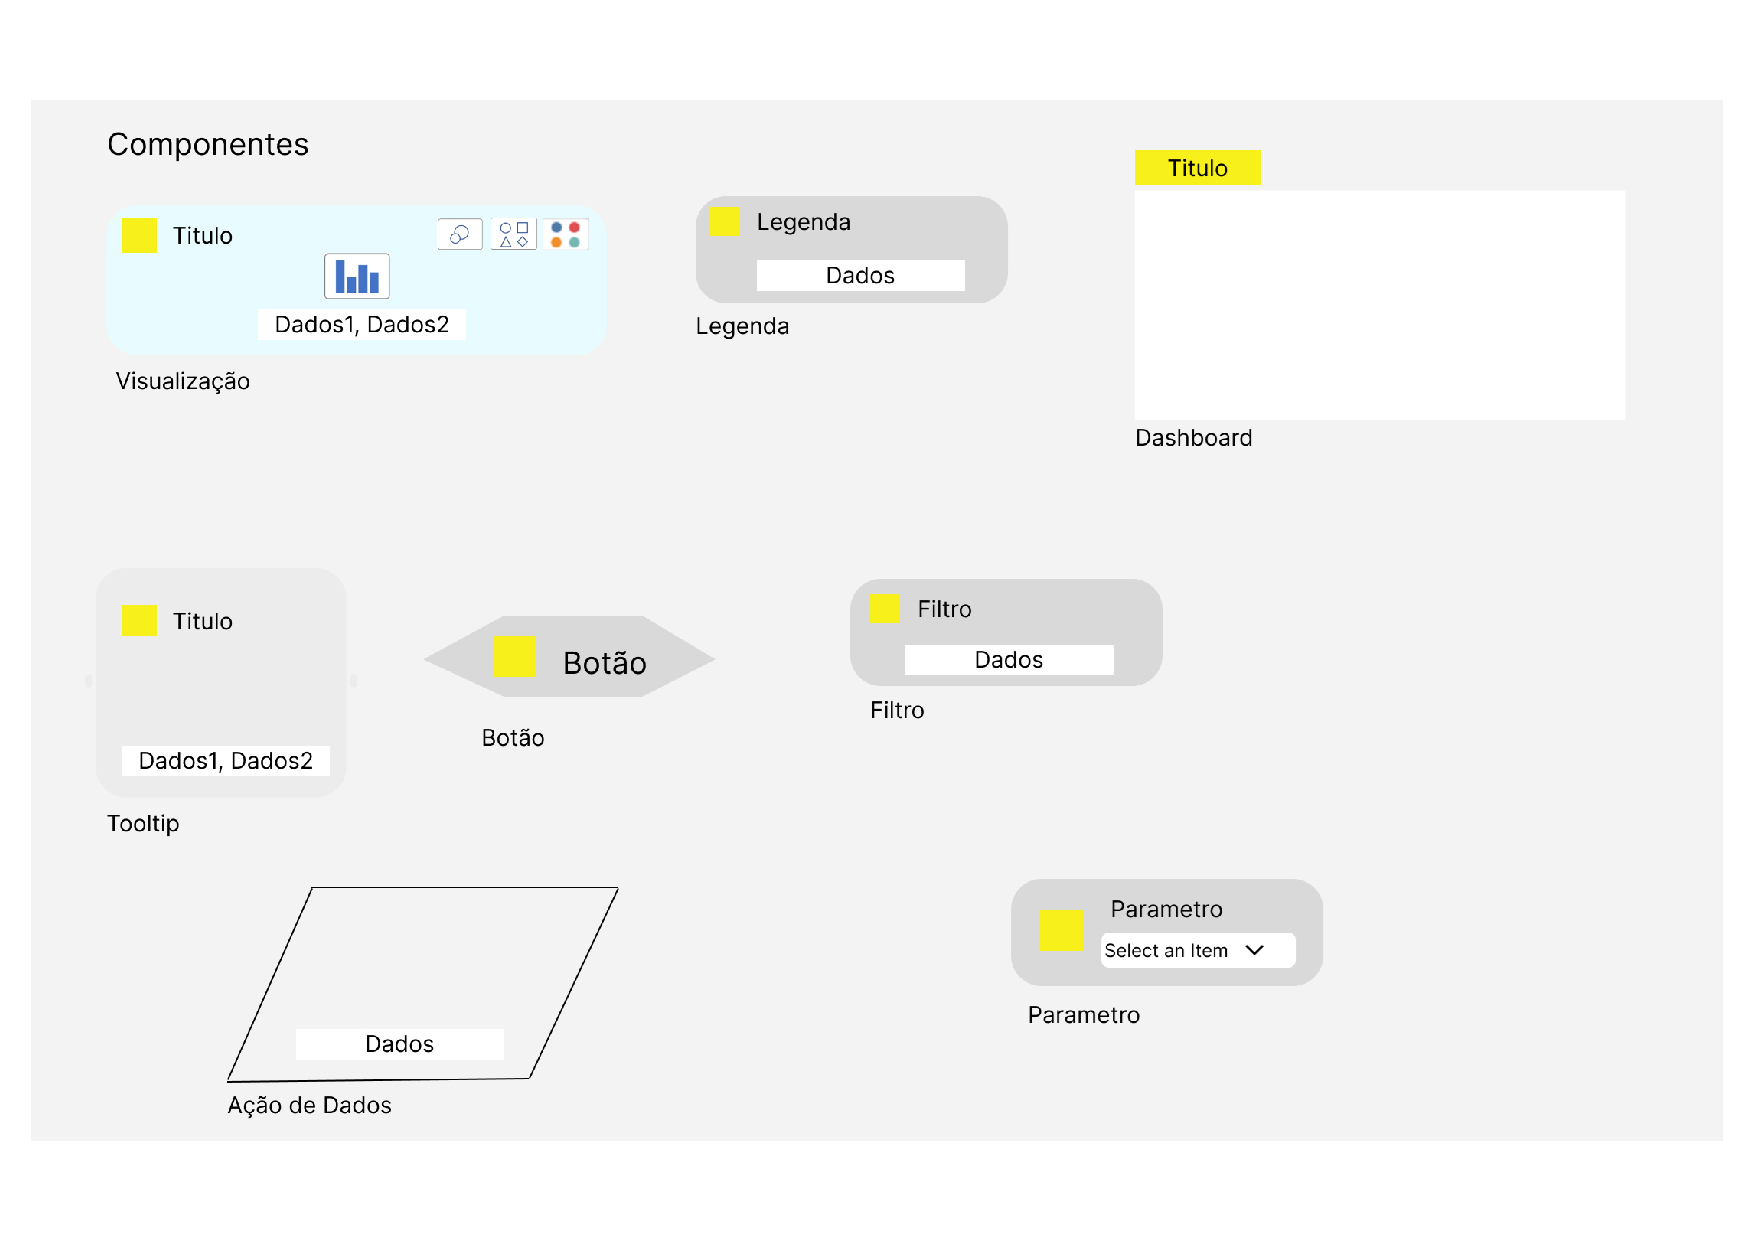
\includegraphics[height=4in]{prototipo/prototipo_componentes}
  \centering
  \caption{Protótipo das diferentes componentes.}
  \label{fig:prototipo_componentes}
\end{figure}

\begin{figure}[htbp]
  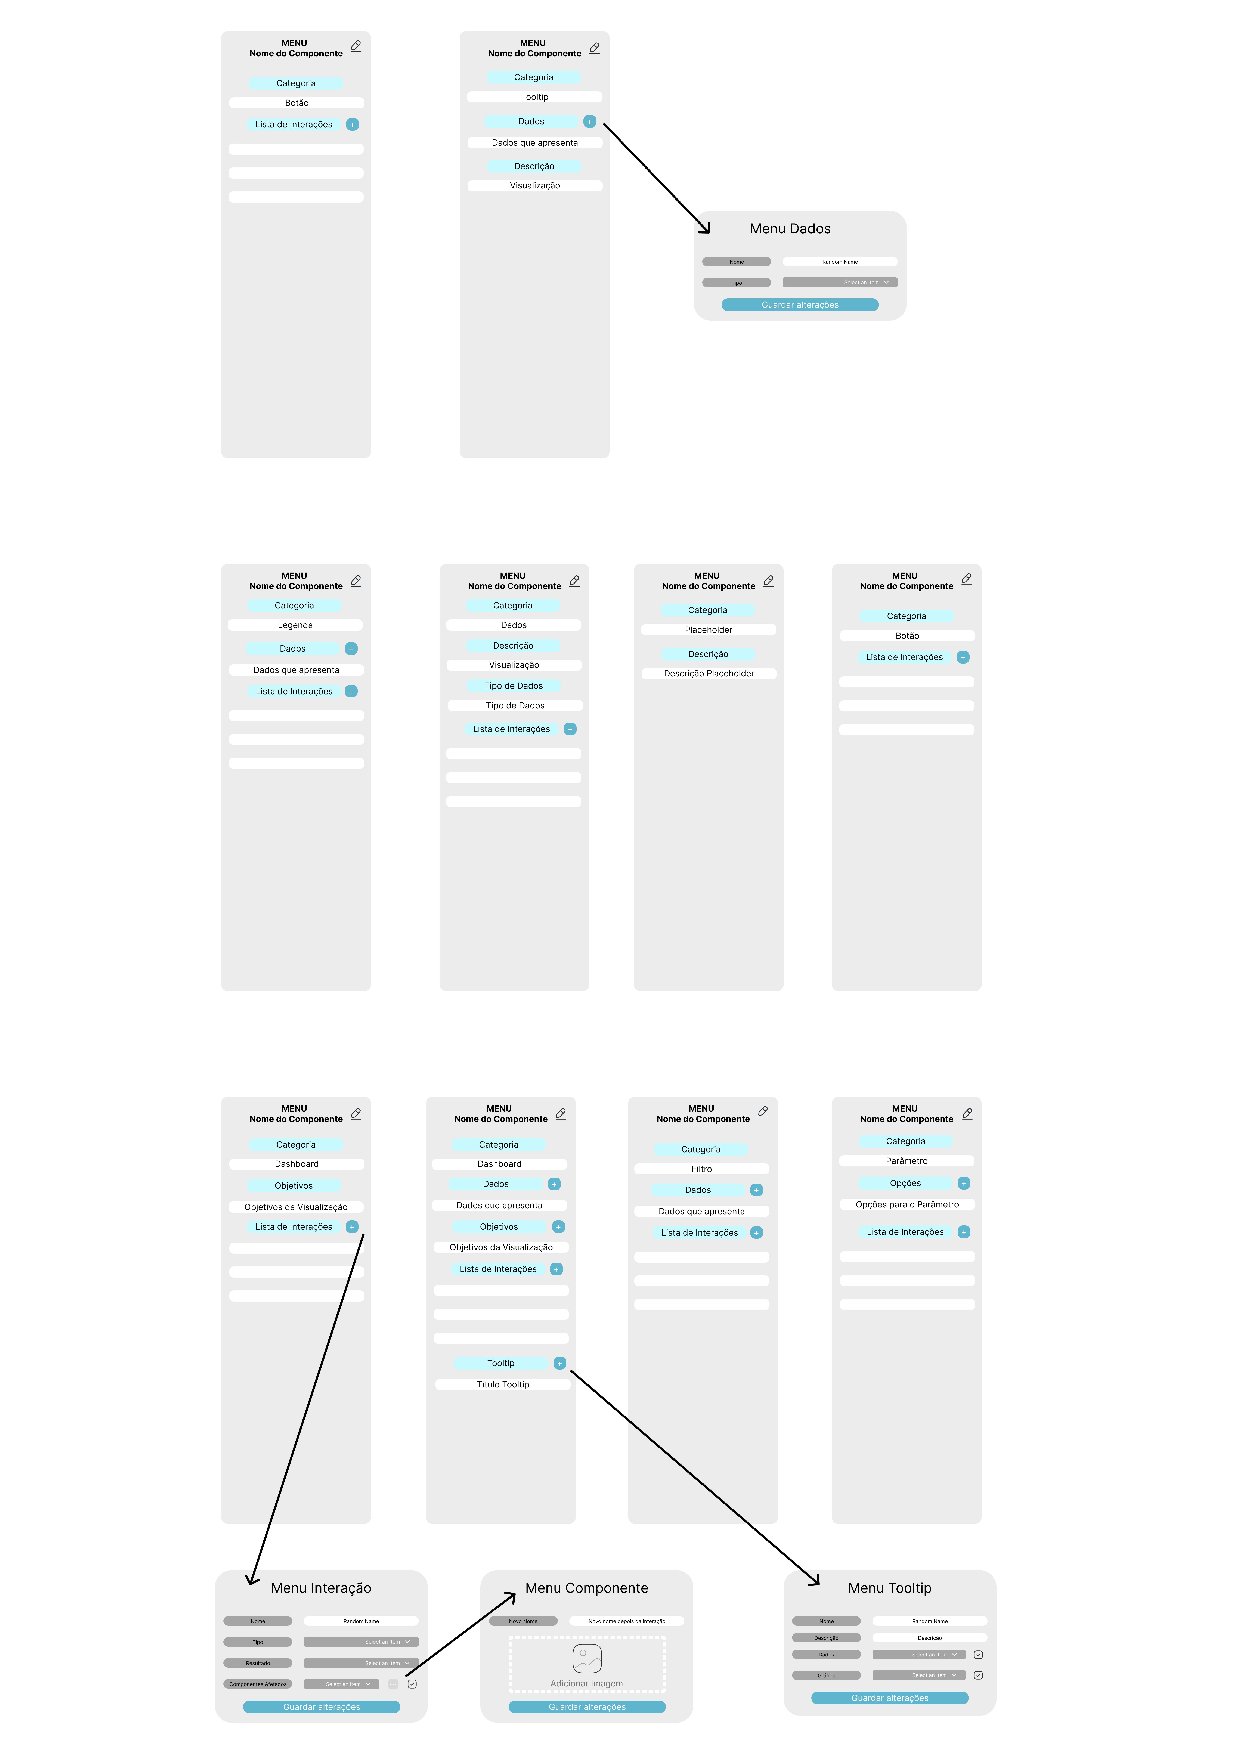
\includegraphics[width=\textwidth]{prototipo/prototipo_menus}
  \centering
  \caption{Protótipo dos diferentes menus de cada componente da solução.}
  \label{fig:prototipo_menus}
\end{figure}